\documentclass[letterpaper, 10 pt, conference]{ieeeconf}
  % use above line letter sized paper
%\documentclass[a4paper, 10pt, conference]{ieeeconf}
  % Use this line for a4 paper
%\IEEEoverridecommandlockouts
  % Needed if you want to use the \thanks command
\overrideIEEEmargins
  % Needed to meet printer requirements.
\usepackage[utf8]{inputenc}
\usepackage{fullpage}
\usepackage{graphicx}
\usepackage{amsfonts}
\usepackage{amssymb}
\usepackage{amsmath}
\usepackage{latexsym}
\usepackage{enumerate}
\usepackage{float}
\usepackage[urlcolor=blue,colorlinks=true]{hyperref}
\usepackage{multirow}
\usepackage{leftidx}
\usepackage{url}
\usepackage[margin=1in]{geometry}
\usepackage[backend=bibtex,
style=numeric
%style=alphabetic
%style=reading
]{biblatex}
\addbibresource{Sources.bib}

\title{Conversion of RGB-D Images to Textured Triangle Meshes with GPU}
\author{Dalton Banks, Collin Boots}
\date{Nov 18, 2013}
\begin{document}
   \maketitle

\section{Background} 
Previous work has demonstrated the diverse capabilities of RGBD cameras, from highly accurate 3D surface mapping \cite{KinectFusion} to reliable 3D pose estimation \cite{Endres,Taguchi}. However, many algorithms attempt to store the generated environment as a RGB 3D point cloud, which is not easily adaptable to dynamic environments, is highly memory intensive for large environments, and provides no intuition to higher perception processes about distinct objects beyond a volumetric approximation. By instead extracting meaningful geometry from the RGB-D data in the form of triangle meshes, several advantages can be realized, including:

\begin{enumerate}
\item Greater storage efficiency
\item Ease of manipulation and modification
\item Efficient real-time rendering
\item Geometric representation conducive to low-level object segmentation as well as higher-order object recognition and manipulation tasks
\item Straightforward tradeoff between simplicity and accuracy in mesh resolution.
\end{enumerate}

\section{Project Scope}
For this project, a portion of the full model-generation pipeline (Figure \ref{fig:pipeline}) will be implemented utilizing CUDA/OpenGL-based GPU acceleration.  Each segment of the pipeline has elements which may benefit from GPU acceleration. The red block represets the actual mesh generatation; this is the most complicated part of the pipeline and the main focus of the project. Blue segments are trivial functions, and green blocks represent stretch goals for the project.

\begin{figure}[!ht]
    \centering
    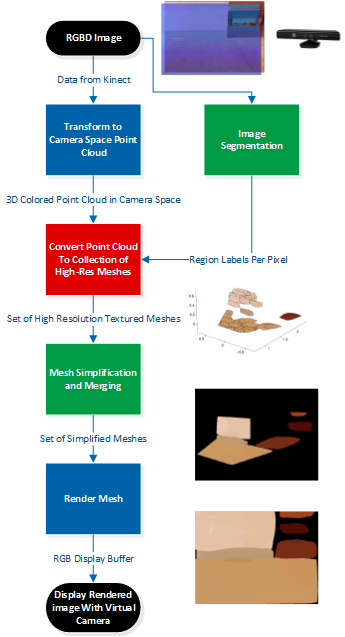
\includegraphics[scale=1.0]{pipelineflowchart.png}
    \caption{Mesh model generation pipeline}
    \label{fig:pipeline}
\end{figure}

\printbibliography
\end{document}
